
\section{MCS Performance on Truth-Selected Muons from numuCC Events in Simulation}\label{MCBNB_performance_section}


% Executive summary
In this section, studies from a truth-selected simulated BNB numuCC \textit{contained} muon sample with {\sc MCTracks} are described. Additionally, similar studies on this sample using automatically reconstructed tracks is described. This section also includes a study justifying that range-based energy is an accurate predictor of true energy for contained muons (with bias less than 1\% and resolution better than 4\%), and therefore can be used in place of true energy so as to compare MC directly to data. The MCS performance on this sample of {\sc MCTracks} is shown to be comparable to that on automatically reconstructed PandoraNuPMA tracks when the track is well reconstructed, with a bias below 5\% and a resolution that varies between 2 and 10\%, performing better for higher momentum (longer) tracks. The resolution is slightly worse for reconstructed tracks than for {\sc MCtracks}. Additionally, the scattering angle of track segments for a given momentum is shown to be similarly gaussian both for {\sc MCTracks} and well reconstructed tracks, in line with the Highland formula prediction. Finally, performance on a sample of \textit{exiting} {\sc MCTracks} and reconstructed tracks is shown.

\subsection{Input Sample}\label{MCBNB_input_sample_section}
The input sample to this portion of the analysis is is 772,000 MCC7 simulated BNB neutrino interactions without any cosmics simulated. These simulated events are run through a fully automated reconstruction chain and then truth information is used to select muons from numuCC interactions which are eligible for MCS analysis. The SAM definition used for this sample is ``prodgenie\_bnb\_nu\_uboone\_mcc7\_reco2''.


\subsection{Fiducial Volume Definition}\label{fidvol_section}
The {\ub} TPC has active volume dimensions of 2.6 m width $\times$ 2.3 m height $\times$ 10.4 m length. For this analysis, a smaller ``fiducial volume'' is defined and referenced throughout this note (for example, in many cases reconstructed tracks are required to be fully contained within the fiducial volume). For reference, the fiducial volume definition used throughout this note is the full TPC volume reduced in by 20 cm from both the cathode plane and the anode wire planes, shifted in 26.5 cm in from both the top and bottom walls of the TPC, shifted in 20 cm from the beam-upstream wall of the TPC, and shifted in 36.8 cm from the downstream wall of the TPC. The reason for this choice of fiducial volume is that it reduces contamination from ``edge effects'' that occur near the walls of the TPC, like electric field distortions and space-charge effects. While the TPC has a total active volume of 62.6 $m^3$, the fiducial volume used in this analysis has a volume of 38.7 $m^3$ or roughly 62\% of the total TPC active volume.









\subsection{Performance with Contained {\sc MCTracks}}\label{MCBNBMCTrack_performance_section}


\subsubsection{MCTrack Description}\label{MCTrack_section}
{\sc MCTrack} objects are made from the output of {\sc geant}4, and are created from {\sc geant}4 energy depositions in the detector. {\sc geant}4 outputs 3D energy depositions in the detector, along with truth information about which parent particles deposited this energy. {\sc MCTracks} are 3D objects which are formed by grouping the energy depositions based on parent particles. Whether a particle in {\sc geant}4 is turned into an {\sc MCTrack} or an {\sc MCShower} (not discussed in this note) is based on truth PDG (for example, muons, protons, and pions always form {\sc MCTracks}).\\

Each {\sc MCTrack} is itself a vector of 3D trajectory points, which are ordered to match the direction of the particle that deposited the energy. Trajectory points are only formed for energy depositions inside of the TPC volume. In general, long {\sc MCTrack}s will have steps separated by up to several centimeters. Each step in an {\sc MCTrack} holds the following information used in this analysis: 3D position, and true energy at that point. Only information within the realm of reconstructable quantities is used in this analysis, with the exception of true energy (which is used for example to quantify a reconstructed energy resolution).\\

Since the output of a nominal reconstruction chain (including hit finding, clustering, matching across planes, etc.) are 3D tracks, {\sc MCTracks} can be studied in an analysis in the exact same way as a reconstructed track would be. {\sc MCTracks} can be thought of as perfectly reconstructed tracks, where each trajectory point along the track is a true 3D energy deposition inside of the {\ub} TPC.\\

Since {\sc MCTracks} are formed from true 3D energy depositions and not from wire signals on drift electrons, {\sc MCTracks} are insensitive to broken wires, noise, and other simulated detector effects.\\

It is worth noting that delta rays eminating from muon tracks are relevant for MCS calculations. Here, delta rays form {\sc MCShowers} and are therefore invisible to this analysis. This is the same as assuming the reconstructed tracks have perfectly removed charge from delta rays in their algorithms.




\subsubsection{Event Selection}\label{MCBNBMCTrack_eventselection_section}
The event selection for this subanalysis is truth based. The fiducial volume used in this subanalysis is the same as is used throughout the note, defined in Section \ref{fidvol_section}. Beginning with the 772,000 events in the sample, the cuts placed are:

\begin{itemize}
\item There is one neutrino interaction in the event (770,241 events remain; some events have two neutrino interactions).
\item The neutrino interaction is of type charged-current (559,348 events remain).
\item The neutrino interaction occurs within the fiducial volume (152,214 events remain) (note the large decrease in statistics because these neutrinos were generated within the full cryostat, and the fiducial volume is much smaller).
\item The interacting neutrino is type $\nu_\mu$ (149,684 events remain).
\item The {\sc MCTrack} associated with the outgoing muon from the interaction is fully contained within the fiducial volume (50,537 events remain).
\item The {\sc MCTrack} associated with the outgoing muon from the interaction is at least one meter in length (23,378 events remain).
\item The {\sc MCTrack} associated with the outgoing muon from the interaction does not decay in flight (this cut is implemented by requiring the {\sc MCTrack}'s total energy at its final trajectory point is equal to the muon mass) (23,342 events remain).
\end{itemize}
After these additional cuts are placed, 23342 events ({\sc MCTracks}) remain for MCS analysis. The energy and angle distributions for these 23342 muons can be seen in Figure \ref{BNBmuon_energy_angle_fig}. It should be noted that any computed metrics from this sample (and therefore any other BNB sample) have convolved any effects of performance differences as a function of angle. While {\sc MCTracks} do not generally suffer from problems related to angle, reconstructed tracks do (since reconstructing 3D tracks that have certain angles with respect to wire planes can be difficult). The effect that reconstructed track angle has on MCS performance is explored briefly in Appendix \ref{AngleStudy_MCBNBRecoTrack_section}.\\

\begin{figure}
\centering
\mbox{
	\subfigure[\textit{Muon energy distribution.}]
	{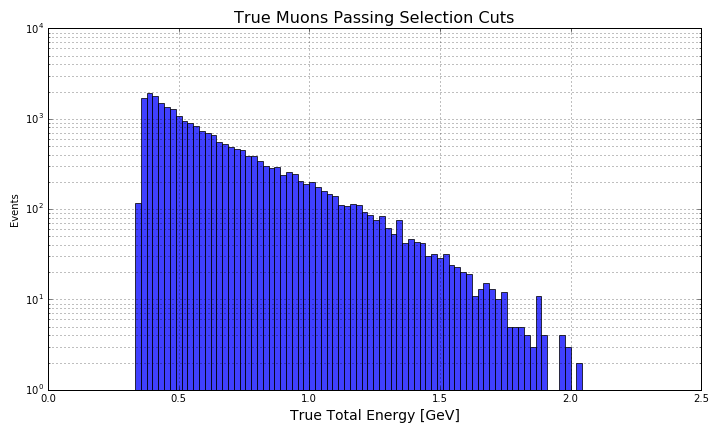
\includegraphics[width=75mm]{Figures/MCBNBMCTrack_EnergySpectrum.png}}
	\quad
	\subfigure[\textit{Muon theta angle (angle with respect to the beam direction) distribution.}]
	{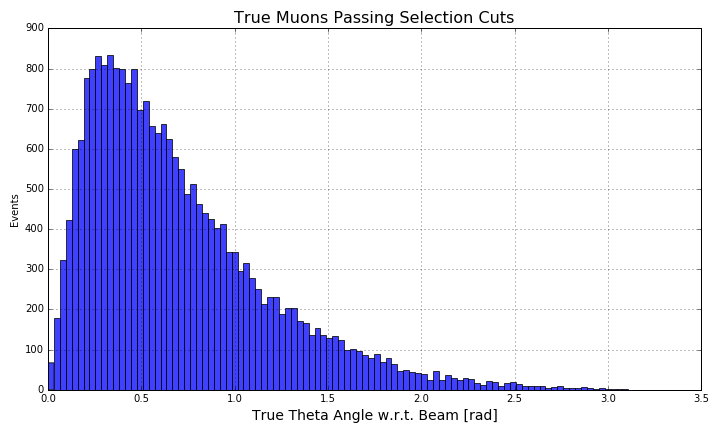
\includegraphics[width=75mm]{Figures/MCBNBMCTrack_AngleSpectrum.png}}
	}
\caption{\textit{Energy and angle distributions for muons from numuCC interactions in {\ub} simulation passing cuts described in Section \ref{MCBNBMCTrack_eventselection_section}.}}
\label{BNBmuon_energy_angle_fig}
\end{figure}



\subsubsection{Range Energy Validation}\label{Range_Energy_Validation_section}
With this sample of {\sc MCTracks}, it is possible to quantify MCS energy (momentum) resolution as a function of true energy (momentum). However, in actual {\ub} data there is obviously no true momentum with which to compare. The additional momentum handle that is used in data for contained tracks is range-based energy. The stopping power of muons in liquid argon is well described by the particle data group\cite{PDG_spline_table}. By using a linear interpolation between points in the cited PDG stopping power table, the start-to-end straight-line length of a track can be used to reconstruct the muon's total energy with good accuracy. Figure \ref{true_range_energy_MCTrack_fig} shows a comparison of range energy to true energy for this sample. \\

In order to compute a bias and a resolution, Figure \ref{true_range_energy_MCTrack_fig} is sliced in bins of true muon energy and a histogram of the fractional energy difference ($\frac{E_{range} - E_{true}}{E_{true}}$) is created for each bin. This distribution is shown for three representative bins in Figure \ref{true_range_bias_resolution_MCTrack_slices_fig}, along with the gaussian fit to each.  The mean ($\mu$) of each gaussian fit is used to compute a bias as a function of true energy, while the width ($\sigma$) of each distribution is used to compute a resolution. Figure \ref{true_range_bias_resolution_MCTrack_fig} shows the bias and resolution for the range-based energy reconstruction method. It can be seen that the bias is negligible and the resolution for this method of energy reconstruction is on the order of 2-4\%. Based on this figure, it is clear that range-based energy (and therefore range-based momentum) is a good handle on the true energy (momentum) of a reconstructed muon track in {\ub} data, assuming that track is well reconstructed in terms of length.

\begin{figure}[ht!]
\begin{center}
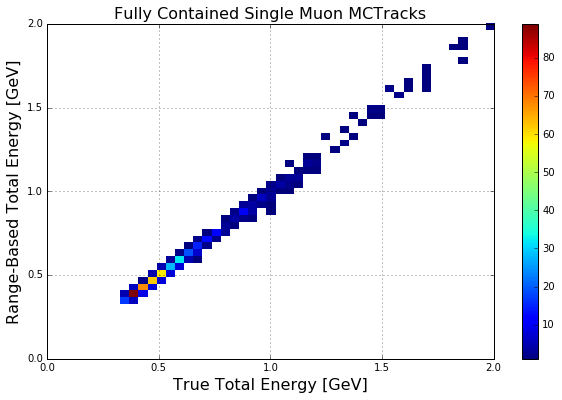
\includegraphics[width=100mm]{Figures/true_range_comparison_MCTracks.png}
\end{center}
\caption{\textit{Range based energy versus true energy for the {\sc MCTrack} sample described in Section \ref{MCBNBMCTrack_eventselection_section}.}}
\label{true_range_energy_MCTrack_fig}
\end{figure}

\begin{figure}
\centering
\mbox{
	\subfigure[\textit{Fractional energy difference between 0.35 and 0.53 GeV true energy.}]
	{\includegraphics[width=50mm]{Figures/{true_range_resolution_MCBNBMCTrack_slice_0.35_0.53}.png}}
	\quad
	\subfigure[\textit{Fractional energy difference between 0.90 and 1.08 GeV true energy.}]
	{\includegraphics[width=50mm]{Figures/{true_range_resolution_MCBNBMCTrack_slice_0.90_1.08}.png}}
	\quad
	\subfigure[\textit{Fractional energy difference between 1.45 and 1.63 GeV true energy.}]
	{\includegraphics[width=50mm]{Figures/{true_range_resolution_MCBNBMCTrack_slice_1.45_1.63}.png}}
	}
\caption{\textit{Fractional energy difference for a few representative bins of true energy derived from Figure \ref{true_range_energy_MCTrack_fig}.}}
\label{true_range_bias_resolution_MCTrack_slices_fig}
\end{figure}




\begin{figure}
\centering
\mbox{
	\subfigure[\textit{Range energy bias as a function of true energy. The vertical error bars are computed as $\frac{\sigma_{fit}}{\sqrt{N}}$, and the horizontal error bars indicate bin width.}]
	{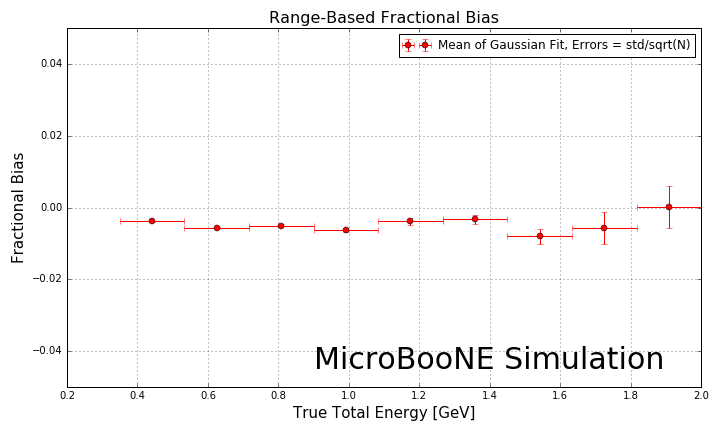
\includegraphics[width=75mm]{Figures/true_range_bias_MCBNBMCTrack.png}}
	\quad
	\subfigure[\textit{Range energy resolution as a function of true energy. The vertical error bars are computed as $\frac{\sigma_{fit}}{\sqrt{2N}}$, and the horizontal error bars indicate bin width.}]
	{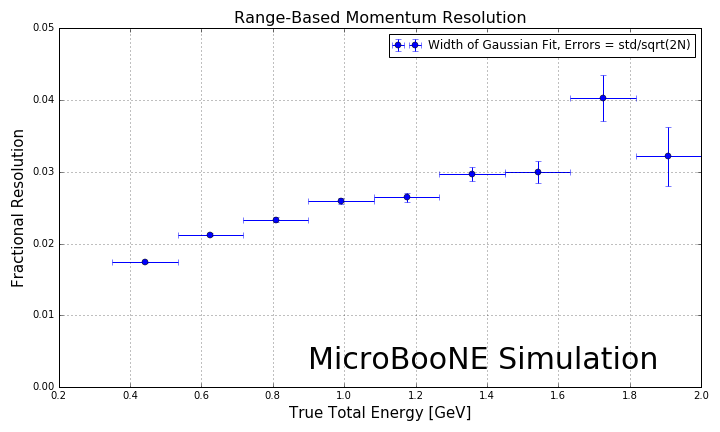
\includegraphics[width=75mm]{Figures/true_range_resolution_MCBNBMCTrack.png}}
	}
\caption{\textit{Range energy and true energy bias and resolution for the {\sc MCTrack} sample described in Section \ref{MCBNBMCTrack_eventselection_section}.}}
\label{true_range_bias_resolution_MCTrack_fig}
\end{figure}







\subsubsection{MCS Momentum Validation}\label{MCS_Momentum_Validation_MCTrack_section}
For this sample of contained {\sc MCTracks}, only the 3D trajectory points of each {\sc MCTrack} are used as input to the MCS code, described in Section \ref{MCS_technique_section}. Note that for {\sc MCTracks}, the detector-inherent angular resolution term $\sigma_o^{res}$ in the Highland formula is set to zero, since {\sc MCTracks} have perfect angular resolution. The resulting MCS momentum versus true momentum can be seen in Figure \ref{MCS_true_momentum_MCTrack_fig}. In order to compute a bias and a resolution, Figure \ref{MCS_true_momentum_MCTrack_fig} is sliced in bins of true momentum and a histogram of the fractional momentum difference ($\frac{p_{MCS}^{-1} - p_{true}^{-1}}{p_{true}^{-1}}$) is created for each bin\footnote{The choice of using inverse momentum is justified in Appendix \ref{inverse_p_justification_section}.}. This distribution is shown for three representative bins in Figure \ref{MCS_true_bias_resolution_MCTrack_slices_fig}, along with the gaussian fit to each.  The mean ($\mu$) of each gaussian fit is used to compute a bias as a function of true momentum, while the width ($\sigma$) of each distribution is used to compute a resolution. The bias and resolution for this momentum reconstruction method shown in Figure \ref{MCS_true_bias_resolution_MCTrack_fig}. This figure indicates a bias in the MCS momentum resolution less than 2.5\%, with a resolution that decreases from about 9\% for contained {\sc MCTracks} with true total momentum around 0.5 GeV (which corresponds to a length of about 1.7 meters) to 4\% for contained {\sc MCTracks} with true total momentum greater than 0.8 GeV (which corresponds to a length of about 3.1 meters). For reference, the bias and resolution as a function of range-based momentum (rather than true-based, as shown) looks much the same, with the resolution decreasing from 9\% to 4\%.


\begin{figure}[ht!]
\begin{center}
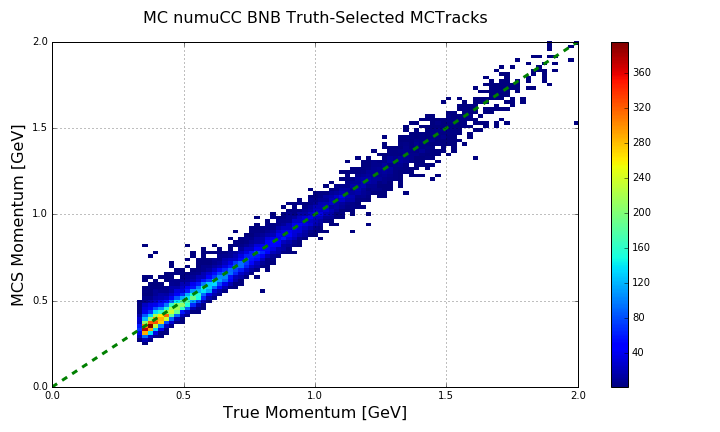
\includegraphics[width=100mm]{Figures/MCS_true_comparison_MCBNBMCTrack.png}
\end{center}
\caption{\textit{MCS computed momentum versus true momentum for the {\sc MCTrack} sample described in Section \ref{MCBNBMCTrack_eventselection_section}. Note the cutoff at around 0.3 GeV true-based momentum is caused by the minimum track length of 100 centimenter requirement.}}
\label{MCS_true_momentum_MCTrack_fig}
\end{figure}

\begin{figure}
\centering
\mbox{
	\subfigure[\textit{Fractional momentum difference between 0.35 and 0.53 GeV true momentum.}]
	{\includegraphics[width=50mm]{Figures/{MCS_true_resolution_MCBNBMCTrack_slice_0.35_0.53}.png}}
	\quad
	\subfigure[\textit{Fractional momentum difference between 0.90 and 1.08 GeV true momentum.}]
	{\includegraphics[width=50mm]{Figures/{MCS_true_resolution_MCBNBMCTrack_slice_0.90_1.08}.png}}
	\quad
	\subfigure[\textit{Fractional momentum difference between 1.45 and 1.63 GeV true momentum.}]
	{\includegraphics[width=50mm]{Figures/{MCS_true_resolution_MCBNBMCTrack_slice_1.45_1.63}.png}}
	}
\caption{\textit{Fractional momentum difference for a few representative bins of true momentum derived from Figure \ref{MCS_true_momentum_MCTrack_fig}.}}
\label{MCS_true_bias_resolution_MCTrack_slices_fig}
\end{figure}


\begin{figure}
\centering
\mbox{
	\subfigure[\textit{MCS momentum bias as a function of true momentum. The vertical error bars are computed as $\frac{\sigma_{fit}}{\sqrt{N}}$, and the horizontal error bars indicate bin width.}]
	{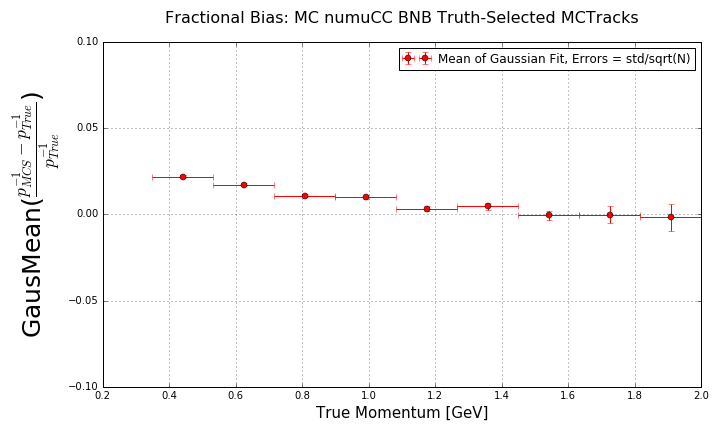
\includegraphics[width=75mm]{Figures/MCS_true_bias_MCBNBMCTrack.png}}
	\quad
	\subfigure[\textit{MCS momentum resolution as a function of true momentum. The vertical error bars are computed as $\frac{\sigma_{fit}}{\sqrt{2N}}$, and the horizontal error bars indicate bin width.}]
	{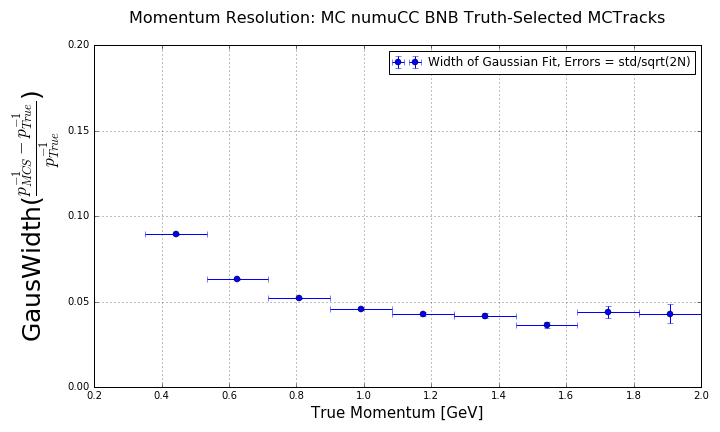
\includegraphics[width=75mm]{Figures/MCS_true_resolution_MCBNBMCTrack.png}}
	}
\caption{\textit{MCS momentum bias and resolution as a function of true momentum for the {\sc MCTrack} sample described in Section \ref{MCBNBMCTrack_eventselection_section}.}}
\label{MCS_true_bias_resolution_MCTrack_fig}
\end{figure}



\subsubsection{Highland Validation}\label{Highland_Validation_MCTrack_section}
For a given track segment momentum and length, 98\% of the angular scatter deviations should be gaussian with an RMS described by the Highland equation (Equation \ref{highland_eqtn}), while the remaining 2\% are larger angle Rutherford scatters\cite{highland}\footnote{This is not actually taken into account explicitly in the current algorithm implementation}. Therefore, a histogram of track segment angular deviations divided by the RMS predicted by the Highland equation should be gaussian with a width of unity. In this section, we validate this claim.\\

For each 14 cm segment of each {\sc MCTrack} in this single muon sample, the momentum of the muon at the start of that segment is estimated by taking the computed MCS momentum and subtracting out momentum lost in the track upstream of the start of this segment as described in Equation \ref{segment_E_equation}. The segment momentum, along with the segment length, is converted into an expected RMS angular deviation by way of Equation \ref{modified_highland_eqtn} with the detector-inherent resolution term set to 0 mrad. For each consecutive pair of segments, the angular scatter in milliradians divided by the Highland expected RMS in millradians is an entry in the histogram shown in Figure \ref{Highland_validation_MCTracks_fig}. From this figure we can see that the Highland formula is valid for {\sc MCTracks}, as the gaussian fit agrees well with the underlying histogram and has a width close to unity.

\begin{figure}[ht!]
\begin{center}
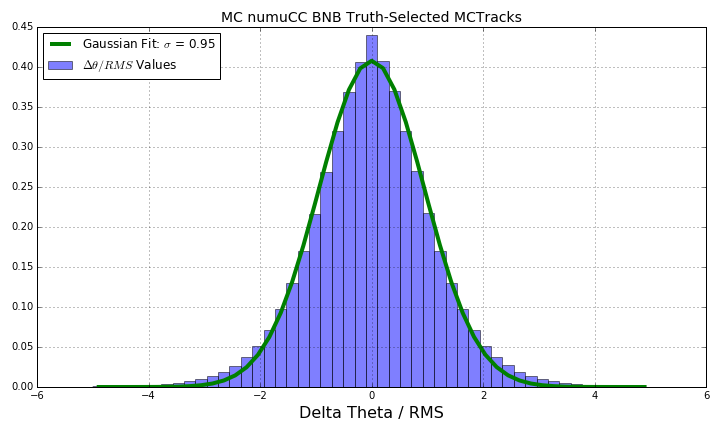
\includegraphics[width=100mm]{Figures/Highland_validation_MCBNBMCTrack.png}
\end{center}
\caption{\textit{14 cm segment angular deviations divided by expected Highland RMS for the single muon {\sc MCTrack} sample described in Section \ref{MCBNBMCTrack_eventselection_section}.}}
\label{Highland_validation_MCTracks_fig}
\end{figure}




























\subsection{Performance with Contained Reconstructed Tracks}\label{MCBNBRecoTrack_performance_section}

\subsubsection{Event Selection}\label{MCBNBRecoTrack_eventselection_section}
The event selection for this subanalysis is identical to that described in Section \ref{MCBNBMCTrack_eventselection_section} with one additional cut. The additional cut is requiring that there is a reconstructed track which starts within 3 cm of the start and ends within 3 cm of the end of the aforementioned {\sc MCTrack} (or vice-versa). This cut is requiring that the track is well reconstructed in terms of position (direction is taken into account later). 13810 events pass this cut, down from the 23342 previously.

\subsubsection{MCS Momentum Validation}\label{MCS_Momentum_Validation_MCBNBRecoTrack_section}
For this sample of reconstructed tracks, only the 3D trajectory points of each reconstructed track are used as input to the MCS code, described in Section \ref{MCS_technique_section}. The detector-inherent resolution term is set to 3 mrad for this analysis, to take into account reconstruction angular resolution. The value of 3 mrad is justified in Appendix \ref{ResolutionStudy_MCBNBRecoTrack_section}. The resulting MCS momentum versus true momentum for this sample of reconstructed tracks without any cuts other than those described in Section \ref{MCBNBRecoTrack_eventselection_section} can be seen in Figure \ref{MCS_true_momentum_MCBNBRecoTrack_fig}. \\

In order to compute a bias and a resolution, Figure \ref{MCS_true_momentum_MCBNBRecoTrack_fig} is sliced in bins of true momentum and a histogram of the fractional momentum difference ($\frac{p_{MCS}^{-1} - p_{true}^{-1}}{p_{true}^{-1}}$) is created for each bin\footnote{The choice of using inverse momentum is justified in Appendix \ref{inverse_p_justification_section}}. This distribution is shown for three representative bins in Figure \ref{MCS_true_bias_resolution_MCBNBRecoTrack_slices_fig}, along with the gaussian fit to each.  The mean ($\mu$) of each gaussian fit is used to compute a bias as a function of true momentum, while the width ($\sigma$) of each distribution is used to compute a resolution. The bias and resolution for this momentum reconstruction method shown in Figure \ref{MCS_true_bias_resolution_MCBNBRecoTrack_fig}. This figure indicates a bias on the order of a few percent, with a resolution that decreases from about 9\% for contained tracks with true total momentum around 0.5 GeV (which corresponds to a length of about 1.7 meters) to below 5\% for contained tracks with true total momentum greater than 0.8 GeV (which corresponds to a length of about 3.1 meters). This agrees well with the analogous plots created from simulated single muons with {\sc MCTracks} (Figure \ref{MCS_true_bias_resolution_MCTrack_fig}).


\begin{figure}[ht!]
\begin{center}
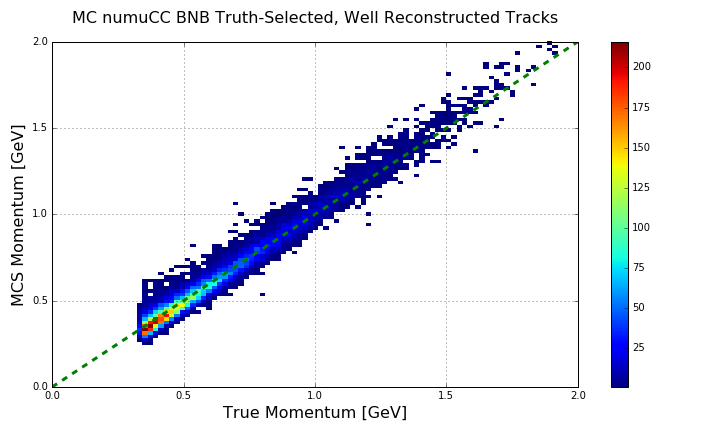
\includegraphics[width=100mm]{Figures/MCS_true_comparison_MCBNBRecoTrack.png}
\end{center}
\caption{\textit{MCS computed momentum versus true momentum for the truth-selected simulated fully contained, well reconstructed muon tracks from numu charged current events.}}
\label{MCS_true_momentum_MCBNBRecoTrack_fig}
\end{figure}


\begin{figure}
\centering
\mbox{
	\subfigure[\textit{Fractional momentum difference between 0.35 and 0.53 GeV true momentum.}]
	{\includegraphics[width=50mm]{Figures/{MCS_true_resolution_MCBNBRecoTrack_slice_0.35_0.53}.png}}
	\quad
	\subfigure[\textit{Fractional momentum difference between 0.90 and 1.08 GeV true momentum.}]
	{\includegraphics[width=50mm]{Figures/{MCS_true_resolution_MCBNBRecoTrack_slice_0.90_1.08}.png}}
	\quad
	\subfigure[\textit{Fractional momentum difference between 1.45 and 1.63 GeV true momentum.}]
	{\includegraphics[width=50mm]{Figures/{MCS_true_resolution_MCBNBRecoTrack_slice_1.45_1.63}.png}}
	}

\caption{\textit{Fractional momentum difference for a few representative bins of true momentum derived from Figure \ref{MCS_true_momentum_MCBNBRecoTrack_fig}.}}
\label{MCS_true_bias_resolution_MCBNBRecoTrack_slices_fig}
\end{figure}


\begin{figure}
\centering
\mbox{
	\subfigure[\textit{MCS momentum bias as a function of true momentum. The vertical error bars are computed as $\frac{\sigma_{fit}}{\sqrt{N}}$, and the horizontal error bars indicate bin width.}]
	{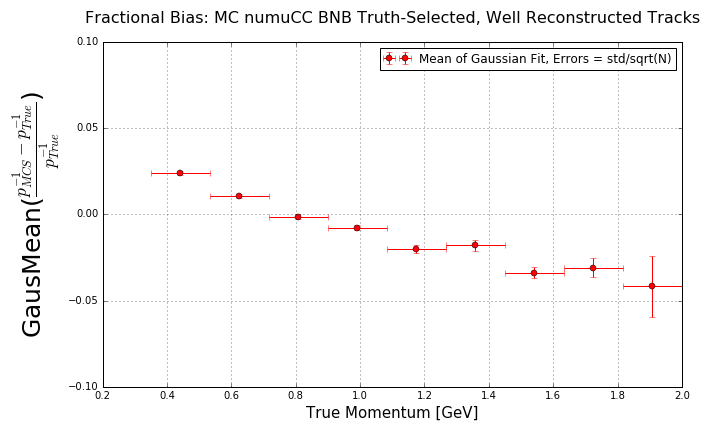
\includegraphics[width=75mm]{Figures/MCS_true_bias_MCBNBRecoTrack.png}}
	\quad
	\subfigure[\textit{MCS momentum resolution as a function of true momentum. The vertical error bars are computed as $\frac{\sigma_{fit}}{\sqrt{2N}}$, and the horizontal error bars indicate bin width.}]
	{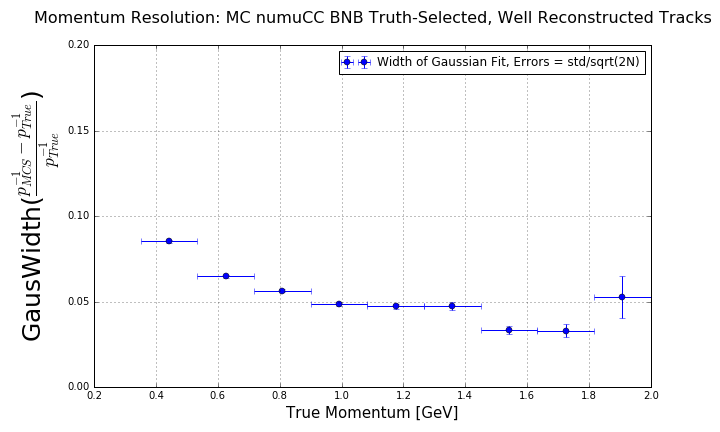
\includegraphics[width=75mm]{Figures/MCS_true_resolution_MCBNBRecoTrack.png}}
	}
\caption{\textit{MCS momentum bias and resolution as a function of true momentum for the truth-selected simulated fully contained, well reconstructed muon tracks from numu charged current events.}}
\label{MCS_true_bias_resolution_MCBNBRecoTrack_fig}
\end{figure}



\subsubsection{Highland Validation}\label{Highland_Validation_MCBNBRecoTrack_section}
For this sample of tracks, the same Highland validation plot is created in exactly the same way as described in Section \ref{Highland_Validation_MCTrack_section}. For each consecutive pair of segments, the angular scatter in milliradians divided by the Highland expected RMS in millradians is an entry in the histogram shown in Figure \ref{Highland_validation_MCBNBRecoTrack_fig}. From this figure we can see that the Highland formula is valid for well reconstructed tracks in simulation when 14 cm segments are used.

\begin{figure}[ht!]
\begin{center}
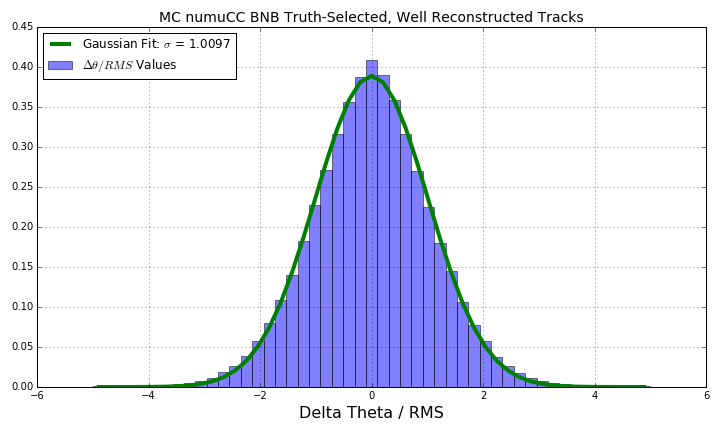
\includegraphics[width=100mm]{Figures/Highland_validation_MCBNBRecoTrack.png}
\end{center}
\caption{\textit{14 cm segment angular deviations divided by expected Highland RMS for the sample of well reconstructed, neutrino induced muons in simulation.}}
\label{Highland_validation_MCBNBRecoTrack_fig}
\end{figure}








\subsection{Performance on Exiting {\sc MCTracks}}\label{ExitingStudy_MCBNBMCTrack_section}
This section describes a study of how the performance of the MCS algorithm changes when exiting {\sc MCTracks} are studied. This is the most important use case of the MCS algorithm, but it is difficult to validate performance in data because there are no other straightforward handles on the particle momenta with which to compare (range energy, calorimetric energy etc. do not accurately represent particle energy when the particle exits the TPC). The input sample for this study was the high statistics simulated BNB neutrino interactions without any cosmics simulated described in Section \ref{MCBNB_input_sample_section}, and this study uses {\sc MCTracks} that have been selected according to the cuts described in Section \ref{MCBNBMCTrack_eventselection_section} while requiring that the {\sc MCTrack} \textit{exits} the fiducial volume rather than is contained inside of it. Note that studying {\sc MCTracks} decouples any effects of track reconstruction or any spacecharge ``edge'' effects ({\sc MCTracks} are insensitive to both of these things). Bias and resolutions will be computed with respect to the true momentum of the muon, since using range-based momentum is not valid for exiting tracks. Note that for {\sc MCTracks}, the detector-inherent angular resolution term $\sigma_o^{res}$ in the Highland formula is set to zero, since {\sc MCTracks} have perfect angular resolution. For exiting tracks, the x- axis for bias and resolution plots is no longer one-to-one with length of track analyzed (as was the case when the x- axis is range-based momentum). Therefore, bias and resolution plots will be broken up into subsamples with different lengths of track contained. Also plots will extend to 4 GeV momenta, which is beyond the momentum range for contained tracks in the fiducial volume.\\

A plot of MCS momentum versus true momentum for this sample of exiting muon {\sc MCTracks} is shown in Figure \ref{MCS_true_momentum_exiting_MCTrack_fig}. The distribution of ($\frac{p_{MCS}^{-1} - p_{true}^{-1}}{p_{true}^{-1}}$) is shown for three representative bins in Figure \ref{MCS_true_exiting_resolution_MCBNBMCTrackExiting_slices_fig}, along with the gaussian fit to each.\\

The bias and resolution plots as a function of true momentum are shown in Figures \ref{exitingMCTrack_bias_fig_alllengths} and \ref{exitingMCTrack_resolution_fig_alllengths} respectively. It can be seen that the bias is below 3\% for all momenta, and the resolution is flat at around 12\%. The bias and resolution plots subdivided in bins of track length analyzed are shown in Figures \ref{exitingMCTrack_bias_fig} and \ref{exitingMCTrack_resolution_fig} respectively. The resolution improves when longer portions of the track are contained in the TPC. Improving with length of track intuitively makes sense; the longer portion of track contained, the more angular scattering measurements can be made to improve the likelihood. The distribution of track lengths in this sample of exiting {\sc MCTracks} is shown in Figure \ref{exitingMCTrack_tracklength_fig}.\\

\begin{figure}[ht!]
\begin{center}
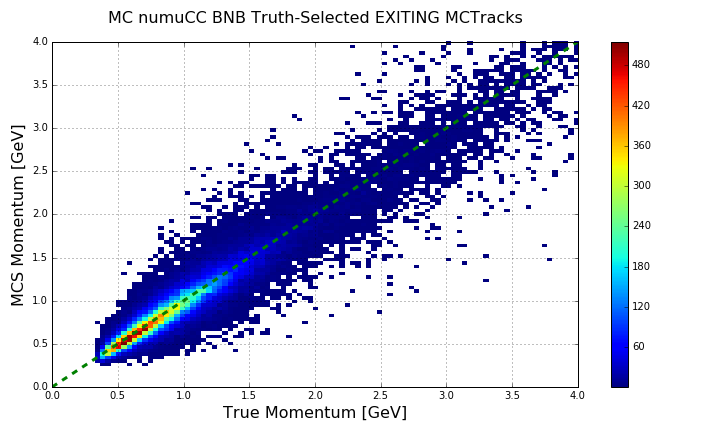
\includegraphics[width=100mm]{Figures/true_MCS_comparison_MCBNBMCTrackExiting.png}
\end{center}
\caption{\textit{MCS computed momentum versus true momentum for the exiting {\sc MCTrack} sample described in Section \ref{ExitingStudy_MCBNBMCTrack_section}.}}
\label{MCS_true_momentum_exiting_MCTrack_fig}
\end{figure}


\begin{figure}
\centering
\mbox{
	\subfigure[\textit{Fractional momentum difference between 0.35 and 0.76 GeV true momentum.}]
	{\includegraphics[width=50mm]{Figures/{MCS_true_exiting_resolution_MCBNBMCTrackExiting_slice_0.35_0.76}.png}}
	\quad
	\subfigure[\textit{Fractional momentum difference between 1.97 and 2.38 GeV true momentum.}]
	{\includegraphics[width=50mm]{Figures/{MCS_true_exiting_resolution_MCBNBMCTrackExiting_slice_1.97_2.38}.png}}
	\quad
	\subfigure[\textit{Fractional momentum difference between 3.59 and 4.00 GeV true momentum.}]
	{\includegraphics[width=50mm]{Figures/{MCS_true_exiting_resolution_MCBNBMCTrackExiting_slice_3.59_4.00}.png}}
	}

\caption{\textit{Fractional momentum difference for a few representative bins of true momentum derived from Figure \ref{MCS_true_momentum_exiting_MCTrack_fig}.}}
\label{MCS_true_exiting_resolution_MCBNBMCTrackExiting_slices_fig}
\end{figure}


\begin{figure}
\centering
\mbox{
	\subfigure[\textit{MCS momentum bias. The vertical error bars are computed as $\frac{\sigma_{fit}}{\sqrt{N}}$, and the horizontal error bars indicate bin width.}\label{exitingMCTrack_bias_fig_alllengths}]
	{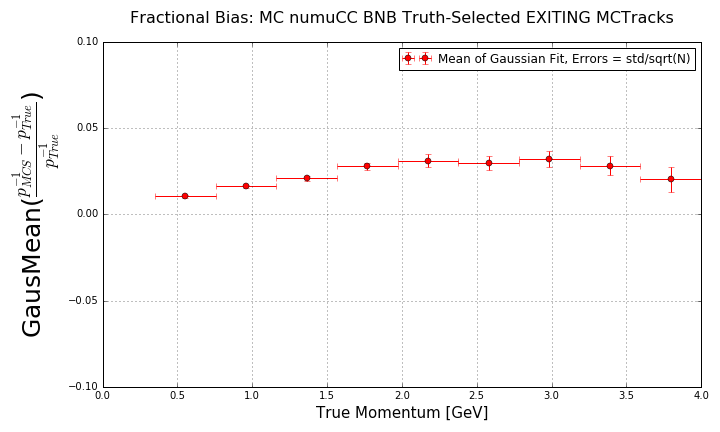
\includegraphics[width=75mm]{Figures/MCS_true_exiting_bias_MCBNBMCTrackExiting.png}}
	\quad
	\subfigure[\textit{MCS momentum resolution. The vertical error bars are computed as $\frac{\sigma_{fit}}{\sqrt{2N}}$, and the horizontal error bars indicate bin width.}\label{exitingMCTrack_resolution_fig_alllengths}]
	{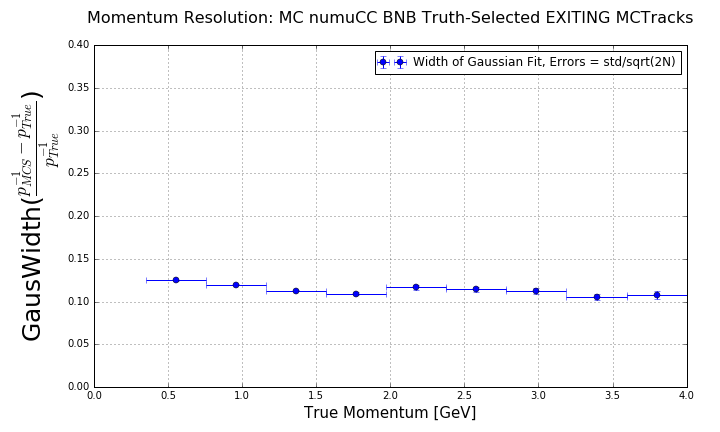
\includegraphics[width=75mm]{Figures/MCS_true_exiting_resolution_MCBNBMCTrackExiting.png}}
	}
\caption{\textit{MCS momentum bias as a function of true momentum for this sample of exiting muon {\sc MCTracks}. The vertical error bars are computed as $\frac{\sigma_{fit}}{\sqrt{N}}$, and the horizontal error bars indicate bin width.}}
\end{figure}



\begin{figure}
\centering
\mbox{
	\subfigure[\textit{MCS momentum bias. The vertical error bars are computed as $\frac{\sigma_{fit}}{\sqrt{N}}$, and the horizontal error bars indicate bin width.}\label{exitingMCTrack_bias_fig}]
	{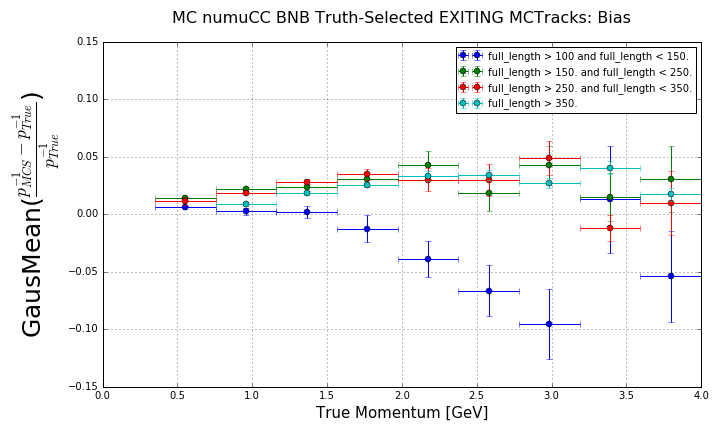
\includegraphics[width=75mm]{Figures/MCS_true_bias_lengthstudy_MCBNBMCTrackExiting.png}}
	\quad
	\subfigure[\textit{MCS momentum resolution. The vertical error bars are computed as $\frac{\sigma_{fit}}{\sqrt{2N}}$, and the horizontal error bars indicate bin width.}\label{exitingMCTrack_resolution_fig}]
	{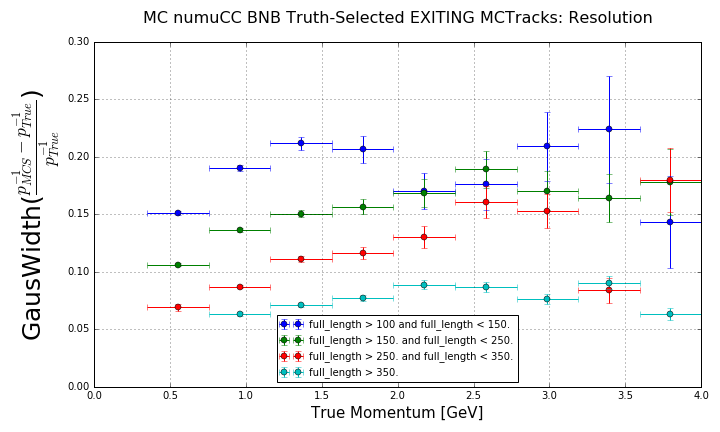
\includegraphics[width=75mm]{Figures/MCS_true_resolution_lengthstudy_MCBNBMCTrackExiting.png}}
	}
\caption{\textit{MCS momentum bias as a function of true momentum for this sample of exiting muon {\sc MCTracks}, subdivided in bins of track length contained. The vertical error bars are computed as $\frac{\sigma_{fit}}{\sqrt{N}}$, and the horizontal error bars indicate bin width.}}
\end{figure}



\begin{figure}[ht!]
\begin{center}
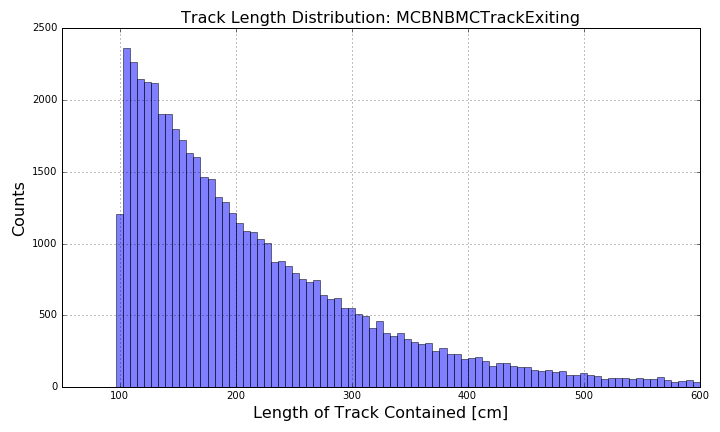
\includegraphics[width=100mm]{Figures/track_length_distribution_MCBNBMCTrackExiting.png}
\end{center}
\caption{\textit{Distribution of track lengths for this sample of exiting muon {\sc MCTracks} described in Section \ref{ExitingStudy_MCBNBMCTrack_section}.}}
\label{exitingMCTrack_tracklength_fig}
\end{figure}





\subsection{Performance on Exiting Reconstructed Tracks}\label{ExitingStudy_MCBNBRecoTrack_section}
This section describes a study of how the performance of the MCS algorithm changes when exiting reconstructed are studied. The input sample for this study was the high statistics simulated BNB neutrino interactions without any cosmics simulated described in Section \ref{MCBNB_input_sample_section}, and this study uses reconstructed tracks that have been selected according to the cuts described in Section \ref{MCBNBRecoTrack_eventselection_section} while requiring that the {\sc MCTrack} to which the reconstructed track is matched \textit{exits} the fiducial volume rather than is contained inside of it. It is important to note that this simulation does not include space charge effects which may introduce a bias to the MCS momentum measurement (space charge ``bends'' tracks, which will cause the MCS algorithm to underestimate the energy). Truncating tracks to be only contained within the fiducial volume (which removes regions with the largest space charge effect) may mitigate the impact space charge has on the algorithm, but this is left for a future study. Note that for reconstructed tracks, the detector-inherent angular resolution term $\sigma_o^{res}$ in the Highland formula is set to 3 mrad, as justified in Appendix \ref{ResolutionStudy_MCBNBRecoTrack_section}. For exiting tracks, the x- axis for bias and resolution plots is no longer one-to-one with length of track analyzed (as was the case when the x- axis is range-based momentum). Therefore, bias and resolution plots will be broken up into subsamples with different lengths of track contained. Also plots will extend to 4 GeV momenta, which is beyond the momentum range for contained tracks in the fiducial volume.\\

A plot of MCS momentum versus true momentum for this sample of exiting muon reconstructed tracks is shown in Figure \ref{MCS_true_momentum_exiting_RecoTrack_fig}. There are some clear tails in which the MCS momentum is an underestimation of the true momentum. The distribution of ($\frac{p_{MCS}^{-1} - p_{true}^{-1}}{p_{true}^{-1}}$) is shown for three representative bins in Figure \ref{MCS_true_exiting_resolution_MCBNBRecoTrackExiting_slices_fig}, along with the gaussian fit to each. The low momentum tails of these distribution can be seen outside of the central gaussian fit.\\

The bias and resolution plots as a function of true momentum are shown in Figures \ref{exitingRecoTrack_bias_fig_alllengths} and \ref{exitingRecoTrack_resolution_fig_alllengths} respectively. It can be seen that the bias is below 4\% for all momenta, and the resolution is roughly 14\% in the relevant momentum region for BNB numuCC muons (below 2 GeV). The resolution begins to worsen when muon momenta passes about 2.5 GeV because at this point the MCS RMS angular scatter begins to be comparable with the detector resolution term of 3 mrad. The positive bias indicates that the MCS algorithm is underestimating the true momentum of the muon which can be attributed to reconstruction effects (since this bias is smaller for {\sc MCTracks} as shown in Figure \ref{exitingMCTrack_bias_fig}). The bias and resolution plots subdivided in bins of track length analyzed are shown in Figures \ref{exitingRecoTrack_bias_fig} and \ref{exitingRecoTrack_resolution_fig} respectively. Both the bias and resolution improve for longer lengths of track contained, with the bias agreeing with zero for tracks longer than 3.5 meters. Resolution improving with length of track is intuitive; the longer portion of track contained, the more angular scattering measurements can be made to improve the likelihood.\\


\begin{figure}[ht!]
\begin{center}
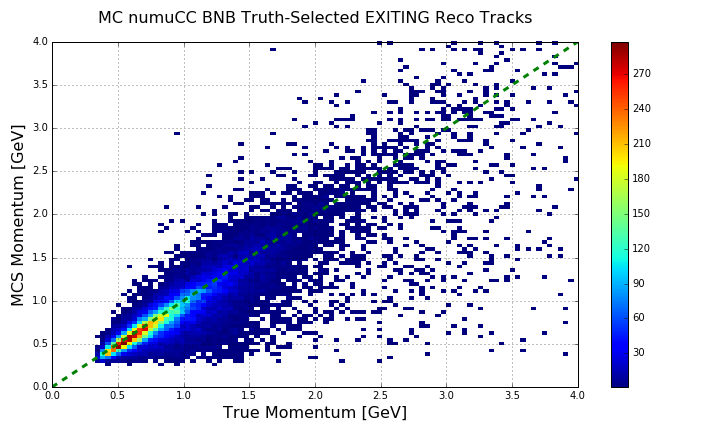
\includegraphics[width=100mm]{Figures/MCS_true_comparison_MCBNBRecoTrackExiting.png}
\end{center}
\caption{\textit{MCS computed momentum versus true momentum for the exiting reconstructed track sample described in Section \ref{ExitingStudy_MCBNBRecoTrack_section}.}}
\label{MCS_true_momentum_exiting_RecoTrack_fig}
\end{figure}


\begin{figure}
\centering
\mbox{
	\subfigure[\textit{Fractional momentum difference between 0.35 and 0.76 GeV true momentum.}]
	{\includegraphics[width=50mm]{Figures/{MCS_true_exiting_resolution_MCBNBRecoTrackExiting_slice_0.35_0.76}.png}}
	\quad
	\subfigure[\textit{Fractional momentum difference between 1.97 and 2.38 GeV true momentum.}]
	{\includegraphics[width=50mm]{Figures/{MCS_true_exiting_resolution_MCBNBRecoTrackExiting_slice_1.97_2.38}.png}}
	\quad
	\subfigure[\textit{Fractional momentum difference between 3.59 and 4.00 GeV true momentum.}]
	{\includegraphics[width=50mm]{Figures/{MCS_true_exiting_resolution_MCBNBRecoTrackExiting_slice_3.59_4.00}.png}}
	}

\caption{\textit{Fractional momentum difference for a few representative bins of true momentum derived from Figure \ref{MCS_true_momentum_exiting_RecoTrack_fig}.}}
\label{MCS_true_exiting_resolution_MCBNBRecoTrackExiting_slices_fig}
\end{figure}


\begin{figure}
\centering
\mbox{
	\subfigure[\textit{MCS momentum bias. The vertical error bars are computed as $\frac{\sigma_{fit}}{\sqrt{N}}$, and the horizontal error bars indicate bin width.}\label{exitingRecoTrack_bias_fig_alllengths}]
	{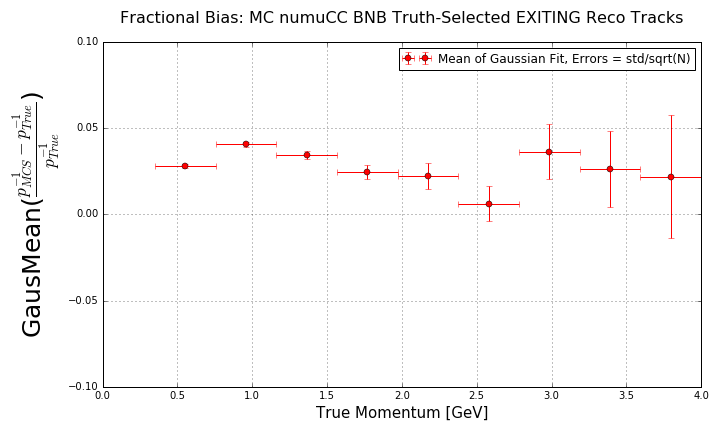
\includegraphics[width=75mm]{Figures/MCS_true_exiting_bias_MCBNBRecoTrackExiting.png}}
	\quad
	\subfigure[\textit{MCS momentum resolution. The vertical error bars are computed as $\frac{\sigma_{fit}}{\sqrt{2N}}$, and the horizontal error bars indicate bin width.}\label{exitingRecoTrack_resolution_fig_alllengths}]
	{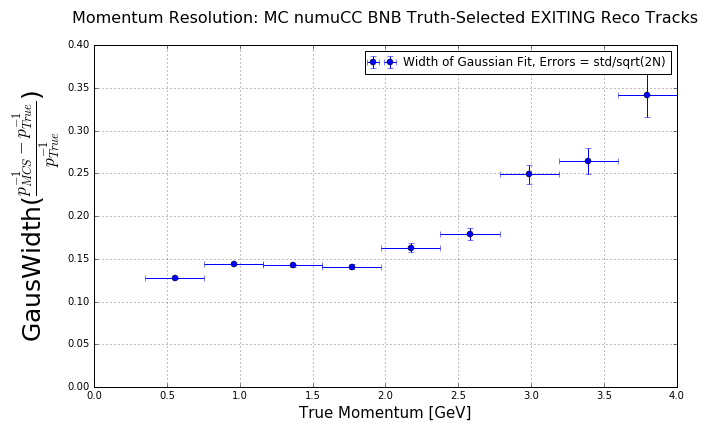
\includegraphics[width=75mm]{Figures/MCS_true_exiting_resolution_MCBNBRecoTrackExiting.png}}
	}
\caption{\textit{MCS momentum bias as a function of true momentum for this sample of exiting muon reconstructed tracks. The vertical error bars are computed as $\frac{\sigma_{fit}}{\sqrt{N}}$, and the horizontal error bars indicate bin width.}}
\end{figure}



\begin{figure}
\centering
\mbox{
	\subfigure[\textit{MCS momentum bias. The vertical error bars are computed as $\frac{\sigma_{fit}}{\sqrt{N}}$, and the horizontal error bars indicate bin width.}\label{exitingRecoTrack_bias_fig}]
	{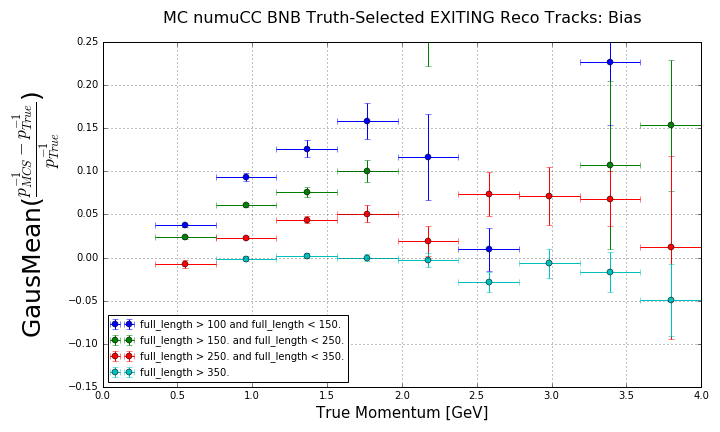
\includegraphics[width=75mm]{Figures/MCS_true_bias_lengthstudy_MCBNBRecoTrackExiting.png}}
	\quad
	\subfigure[\textit{MCS momentum resolution. The vertical error bars are computed as $\frac{\sigma_{fit}}{\sqrt{2N}}$, and the horizontal error bars indicate bin width.}\label{exitingRecoTrack_resolution_fig}]
	{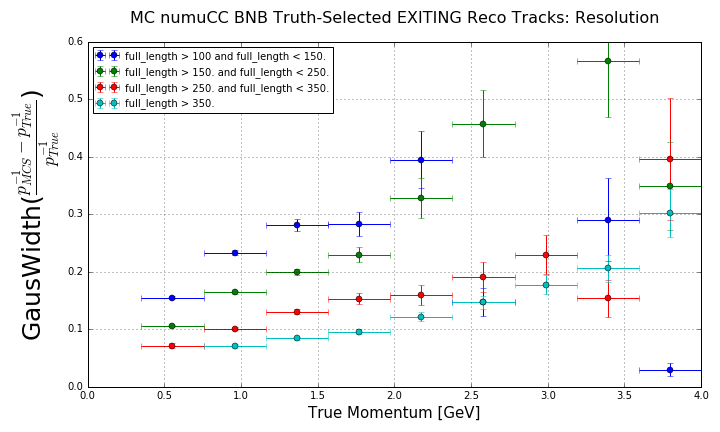
\includegraphics[width=75mm]{Figures/MCS_true_resolution_lengthstudy_MCBNBRecoTrackExiting.png}}
	}
\caption{\textit{MCS momentum bias as a function of true momentum for this sample of exiting muon reconstructed tracks, subdivided in bins of track length contained. The vertical error bars are computed as $\frac{\sigma_{fit}}{\sqrt{N}}$, and the horizontal error bars indicate bin width.}}
\end{figure}


